\documentclass[xcolor=dvipsnames]{beamer}

%\usecolortheme[named=Brown]{structure}
\usecolortheme[RGB={150,150,90}]{structure}

% Preamble

% My footline
%\useoutertheme{infolines}
%\setfootline{\insertshortauthor, \insertshortdate 
%    \hfill slide \insertframenumber/\inserttotalframenumber} 

%\usepackage[latin1]{inputenc}
%\usetheme[height=8mm]{Rochester}
\usetheme{Copenhagen}
%\setbeamercolor{normal text}{bg=red!10}

\hypersetup{colorlinks=true,linkcolor=Brown}
% for hyperlinks

% Customisation of theme...
\setbeamertemplate{items}[ball]  % bullets
\setbeamertemplate{blocks}[rounded][shadow=false] % boxes 
\setbeamertemplate{navigation symbols}{} % to disable the navigation buttons at the bottom

\usepackage{mathrsfs}
\usepackage{latexsym,amssymb}
\usepackage{amsmath}
\usepackage{amstext}
\usepackage{amsfonts}
\usepackage{amssymb}

\newcommand{\Lim}[1]{\raisebox{0.5ex}{\scalebox{0.8}{$\displaystyle \lim_{#1}\;$}}}

\title[Mini Project]{Numerical estimation of tensor power spectrum}
\subtitle{during Inflation.}
\author{Poruri Sai Rahul}
\institute[IITM]{Department of Physics\\
IIT Madras}
\date[June 2015]{\today}

% Begin document
\begin{document}

\begin{frame}[plain,label=cover]
\titlepage
\end{frame}

\begin{frame}{Introduction}

\[ S[\phi] = \int {\rm d}^4x \sqrt{-g}\left[ \left(\frac{1}{2}\right)\left(\partial^{\lambda}\phi \partial_{\lambda}\phi\right) - V(\phi)\right], \]

\[ T^{\mu}_{\nu} = \partial^{\mu}\phi \partial_{\nu}\phi -\delta^{\mu}_{\nu}\left[\left(\frac{1}{2}\right)\left(\partial^{\lambda}\phi \partial_{\lambda}\phi\right) - V(\phi)\right], \]

\[ \ddot{\phi} + 3H\dot{\phi} + V_{\phi} = 0, \]

\[V_{\phi} = \left({\rm d}V/{\rm d}\phi\right)\] \[H = \dot{a}/a\]

\end{frame}

\begin{frame}

\[ T^{0}_{0} = \left(\frac{\dot{\phi}^2}{2}\right) +V(\phi) = \rho, \]

\[ T^{i}_{j} = -\left[\left(\frac{\dot{\phi}^2}{2}\right) - V(\phi)\right]\delta^{i}_{j} = -p\delta^i_j. \]

\[  \dot{H} = \frac{-\dot{\phi}^2}{2M_P^2}, \]

\[ H^2 = \left(\frac{1}{3M_P^2}\right)\left[\frac{\dot{\phi}^2}{2} + V\right]. \]

\[ \phi(t)= \sqrt{2}M_P \int dt \sqrt{-\dot{H}}, \]

\[ V(t) = M_P^2\left(3H^2 + \dot{H}\right). \]

\end{frame}

\begin{frame}

\[ a(t) = a_0t^q. \]

\[ a(\eta) = \left(-\mathcal{\bar{H}}\eta\right)^{\left(\gamma+1\right)}, \]

\[ \mathcal{\bar{H}} = [a_0^{1/q}(q-1)] ~{\rm ~and}~ \gamma  = -\left(\frac{2q-1}{q-1}\right). \]

\[ \frac{\phi(t)}{M_P} =\sqrt{\left(2q\right)} {\rm ln}\left[\sqrt{\left(\frac{V_0}{(3q-1)q}\right)}\left(\frac{t}{M_P}\right)\right], \]

\[ V(\phi) = V_0\exp\left[-\sqrt{\frac{2}{q}}\left(\frac{\phi}{M_P}\right)\right]. \]

\[ \phi(N) = \sqrt{\left(\frac{2}{q}\right)} N - \sqrt{\left(2q\right)}{\rm ln}t_0. \]

\[ H(N) = H_0\exp^{-N/q}. \]

\[  \epsilon_1(N) = \phi'(N)^2/2 = \left(\frac{1}{q}\right), \] 

\end{frame}

\begin{frame}

\[ V(\phi) = V_0 \exp\left[-\sqrt{\frac{2}{q}}\left(\phi - \phi_i\right)\right], \]

\[ \frac{{\rm d}^2\phi}{{\rm d}N^2} + \left[3 - \frac{1}{2}\left(\frac{{\rm d}\phi}{{\rm d}N}\right)^2\right]\frac{{\rm d}\phi}{{\rm d}N} + \left[6 - \left(\frac{{\rm d}\phi}{{\rm d}N}\right)^2\right]\frac{1}{2V(\phi)}\frac{{\rm d}V(\phi)}{{\rm d}N} = 0. \]

\[ H^2 = \frac{2V(\phi)}{3-({\rm d}\phi/{\rm d}N)^2}. \]

\[ \phi = 1, \]

\[ \frac{{\rm d}\phi}{{\rm d}N}_0 = \frac{\sqrt{2q}}{t_0}\frac{1}{H_0}. \]

\end{frame}

\begin{frame}

\[ V = V_0\left[1 - \left(\frac{\phi}{\mu}\right)^p\right], \]

\[p = 4, \mu = 15, V_0 = 5.55702\times10^{-10}\]

\[ \ddot{\phi} + 3\left(\frac{1}{\sqrt{3}M_P}\right)\left[\frac{\dot{\phi}^2}{2} + V\right]\dot{\phi} - \left(\frac{pV_0}{\mu}\right)\left(\frac{\phi}{\mu}\right)^{(p-1)} = 0. \]

\end{frame}

\begin{frame}

\[ \delta G^0_0 = \delta G^0_i = 0, \]

\[ \delta G^i_j = -\left(\frac{1}{2}\right)\left(\ddot{h}_{ij} + 3H\dot{h}_{ij} - \frac{1}{a^2}\nabla ^2h_{ij}\right), \]

\[ \delta T^0_0 = \delta\rho, \]

\[ \delta T^0_i = \left(\nabla_i\delta\sigma\right), \]

\[ \delta T^i_j = -\delta p\delta^i_j. \]

\[\delta T^i_j = 0\]

\[ \ddot{h} + 3H\dot{h} - \left(\frac{1}{a^2}\right)\nabla ^2h = 0. \]

\[ {h}^{''} + 2{\mathcal{H}}{h}^{'} - \left(\frac{1}{a^2}\right)\nabla ^2h = 0. \]

\[ \ddot{h}_k + 3H\dot{h}_k + \left(\frac{k^2}{a^2}\right)h_k = 0. \]

\end{frame}

\begin{frame}

\[
\hat{h}(\eta, {\bf x}) = \int \frac{{\rm d}^3\bf{k}}{(2\pi)^{3/2}} \left[\hat{a_k}h_k(\eta)e^{i\bf{k\cdot x}}+ \hat{a_k}^{\dagger}h_k^{*}(\eta)e^{-i\bf{k\cdot x}}\right] ,
\]

\[
\int^{\infty}_0 {\rm d}k {\mathcal{P}}_T(k) = \int {\rm d}^3{\bf{k}}\int\frac{d^3(\bf{x}-\bf{x'})}{(2\pi)^3}\langle 0|P(\eta,{\bf{x}})P(\eta, {\bf{x'}})|\rangle e^{-i{\bf{\left[k \cdot (x-x')\right]}}},
\]

\[\hat{a_k}|0\rangle = 0 \forall {\bf{k}}\]

\[ {\mathcal{P}}_T(k) = 2 \left(\frac{k^3}{2\pi^2}\right) |h_k|^2, \]
\end{frame}

\begin{frame}

\[ h_k = \left(u_k/a\right) \]

\[ u''_k + \left[k^2 - \left(\frac{a''}{a}\right)\right]u_k = 0, \]

\end{frame}

\begin{frame}

\[ \Lim{\left( k/aH\right) \rightarrow \infty} u_k(\eta) \rightarrow \left(\frac{1}{\sqrt{2k}}\right){\rm e}^{-ik\eta}. \]

\[ u_k(\eta) = \left(\frac{-\pi\eta}{4}\right)^{1/2}{\rm e}^{i[\nu+(1/2)](\pi/2)}{\rm H}_{\nu}^{(1)}(-k\eta), \]

\[ \nu = [\gamma + (1/2)] \]

\[ (-k\eta \rightarrow 0)) \]

\[ {\rm H}_{\nu}^{(1)} \sim -(i/\pi)\Gamma(\nu)(\frac{1}{2}z)^{(-\nu)}. \]

\[ \mathcal{P}_T(k) = A_T\bar{\mathcal{H}}^2\left(\frac{k}{\mathcal{\bar{H}}}\right)^{2(\gamma+2)}, \]

\[ A_T = \left[\frac{1}{\pi^3M_P^2}\right]\left(\frac{|\Gamma(\nu)|^2}{2^{(2\gamma+1)}}\right). \]

\end{frame}

\begin{frame}

\[  \frac{{\rm d}^2h_k}{{\rm d}N^2} +\left (3+\frac{1}{H}\frac{{\rm d}H}{{\rm d}N}\right)\frac{{\rm d}h_k}{{\rm d}N} + \frac{k^2}{a^2H^2}h_k = 0. \]

\[ h_k  = \frac{1}{\sqrt{2k_0}a(N)}, \] 

\[ \frac{{\rm d}h_k}{{\rm d}N} = -\frac{1}{\sqrt{2k_0}a(N)} - \frac{i\sqrt{(k0/2)}}{a^2(N)H(N)}, \] 

\end{frame}

\begin{frame}
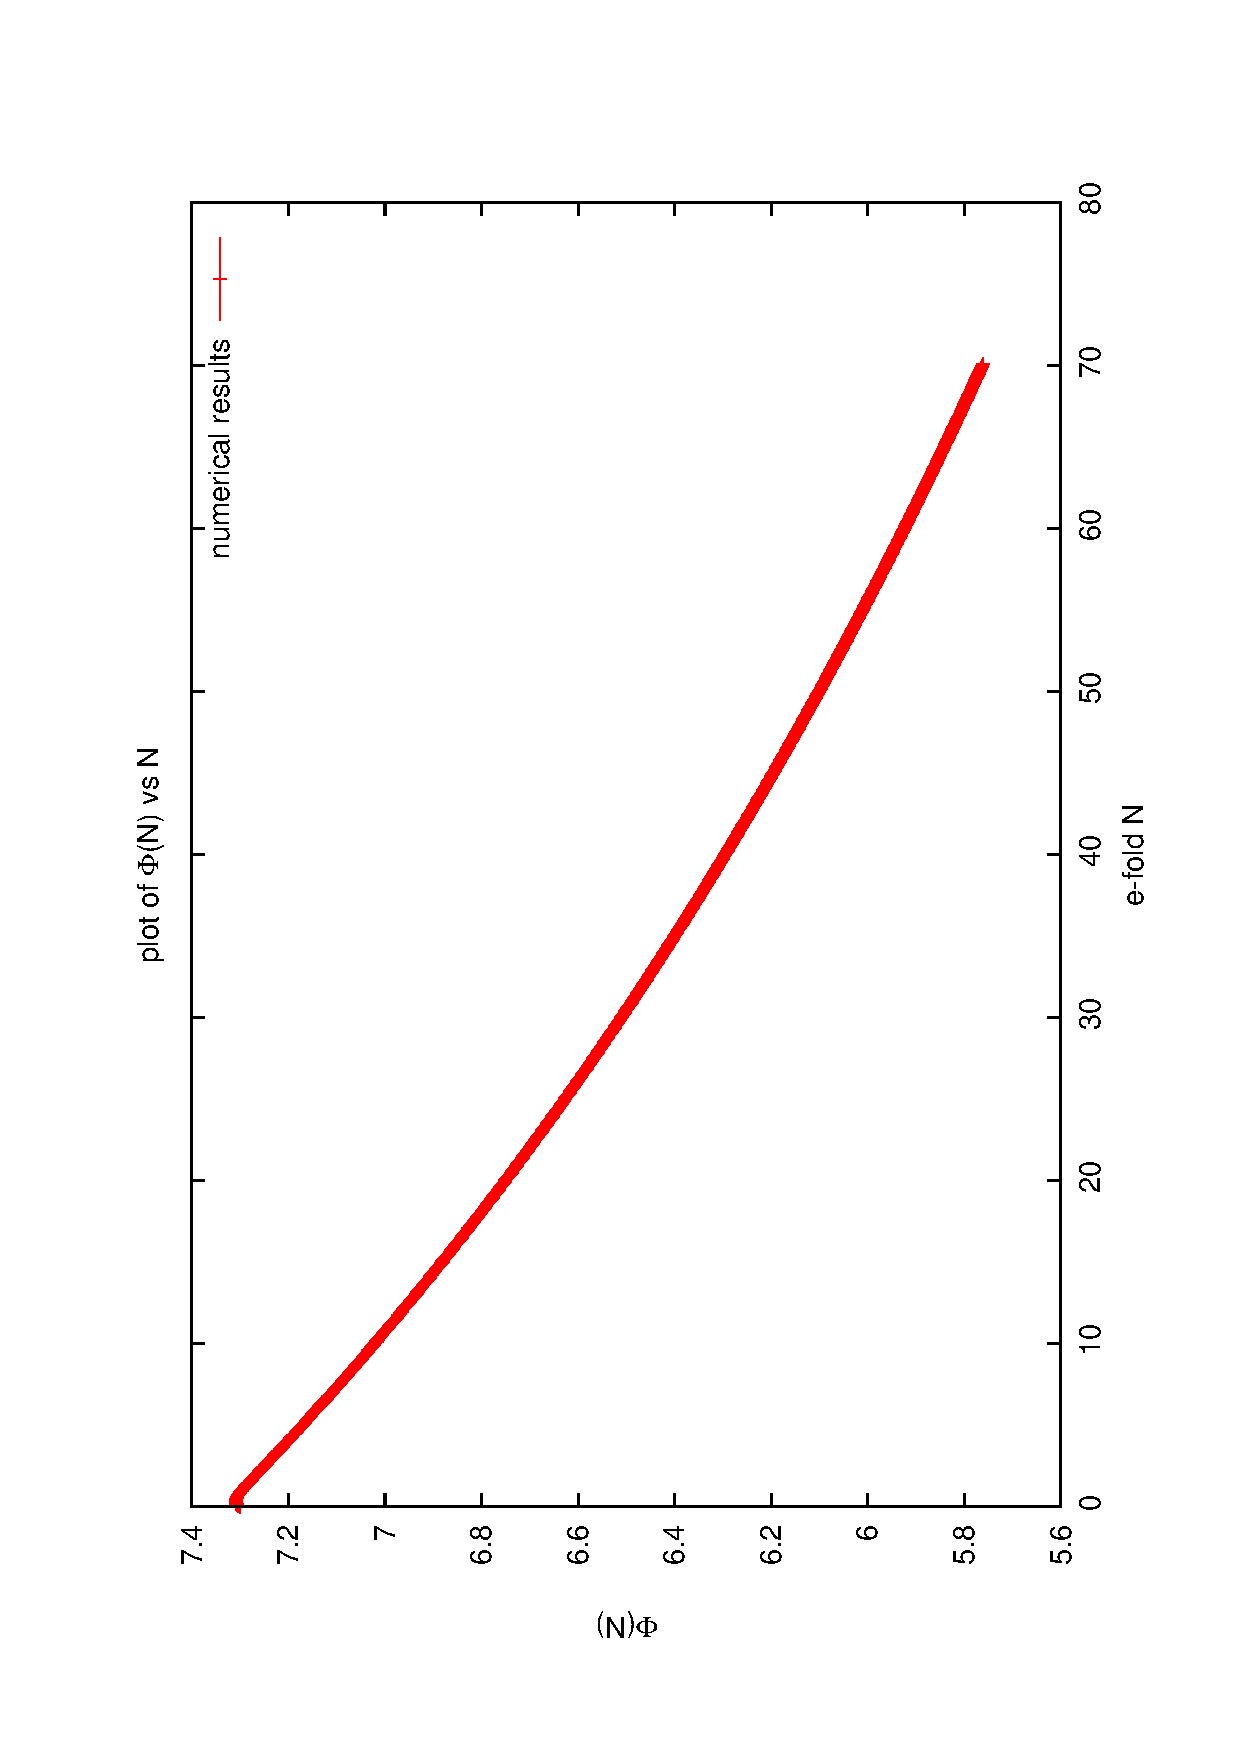
\includegraphics[scale=0.5]{plots/phi_vs_N_small_field.png}
\end{frame}

\begin{frame}
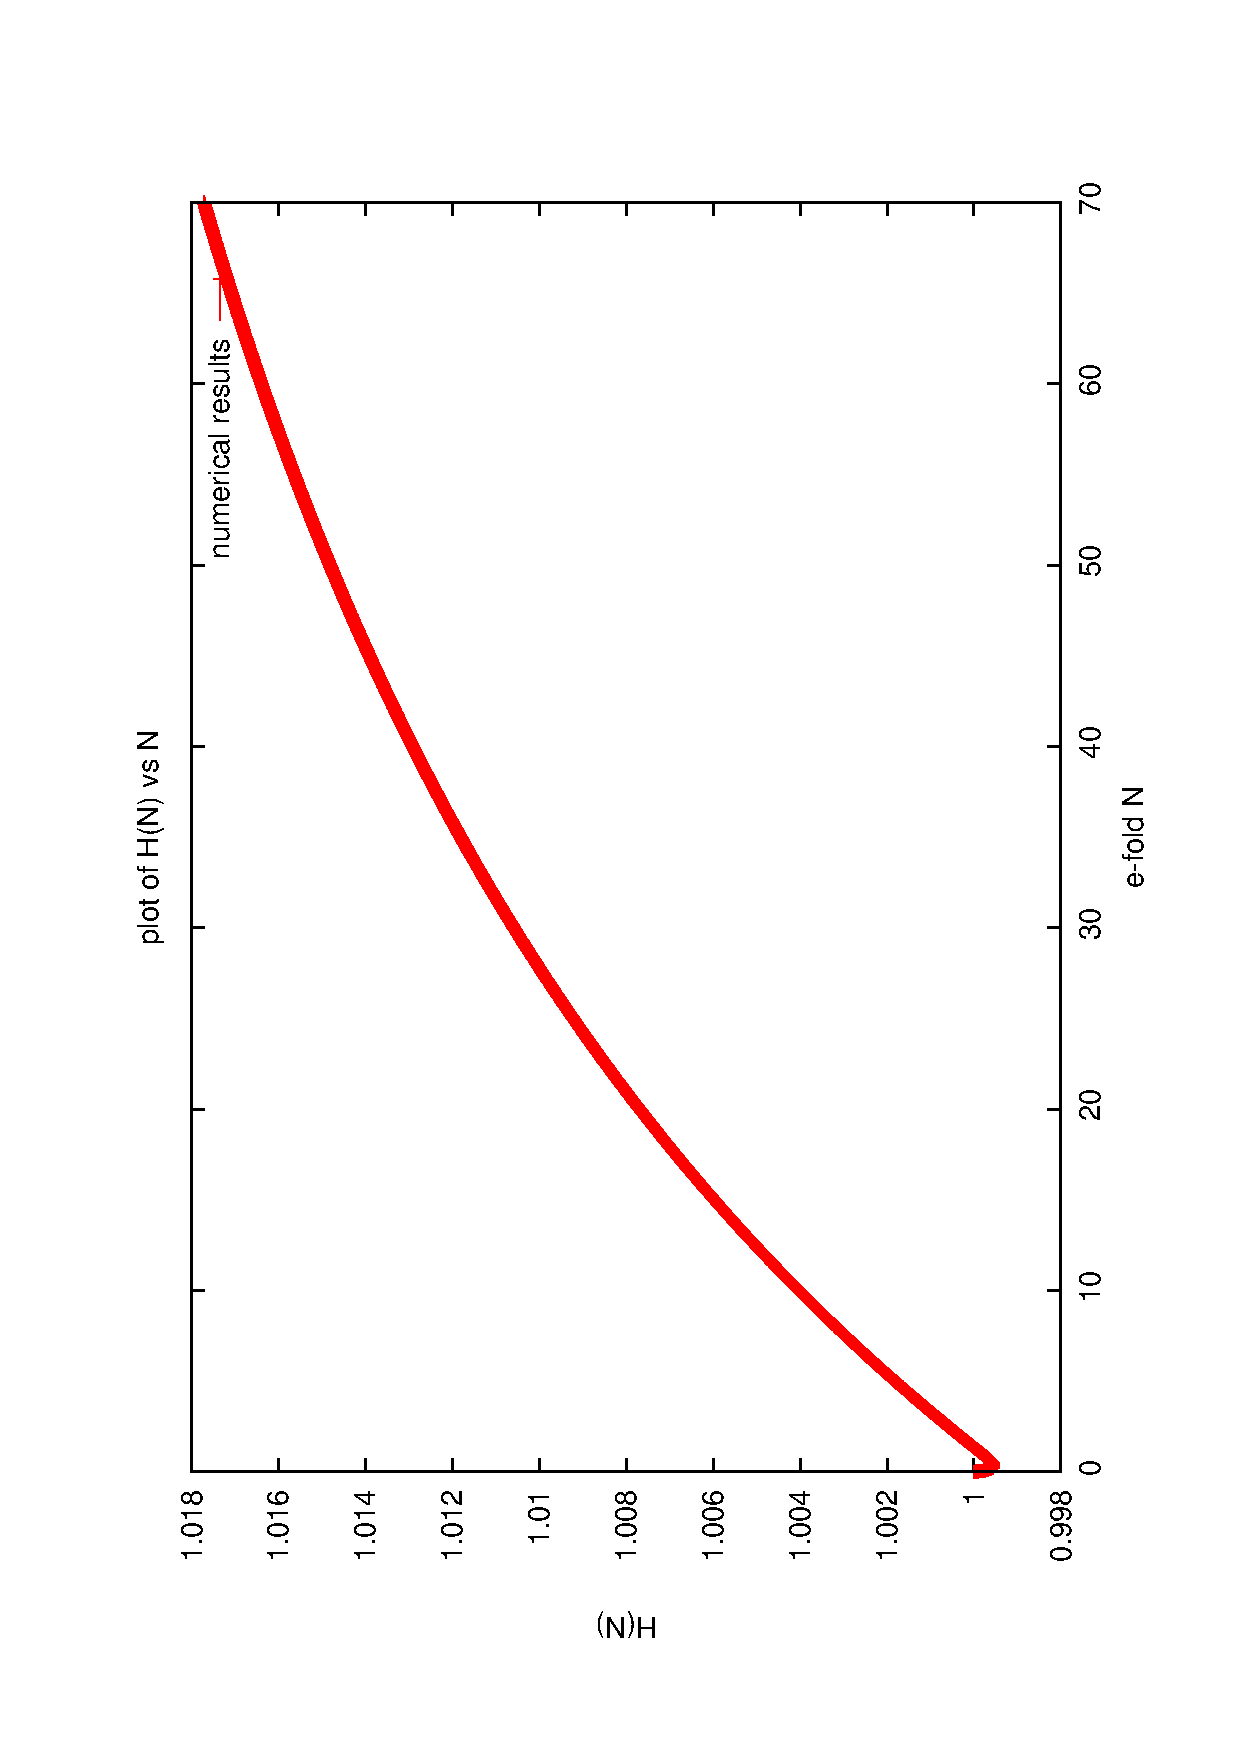
\includegraphics[scale=0.5]{plots/H_vs_N_small_field.png}
\end{frame}

\begin{frame}
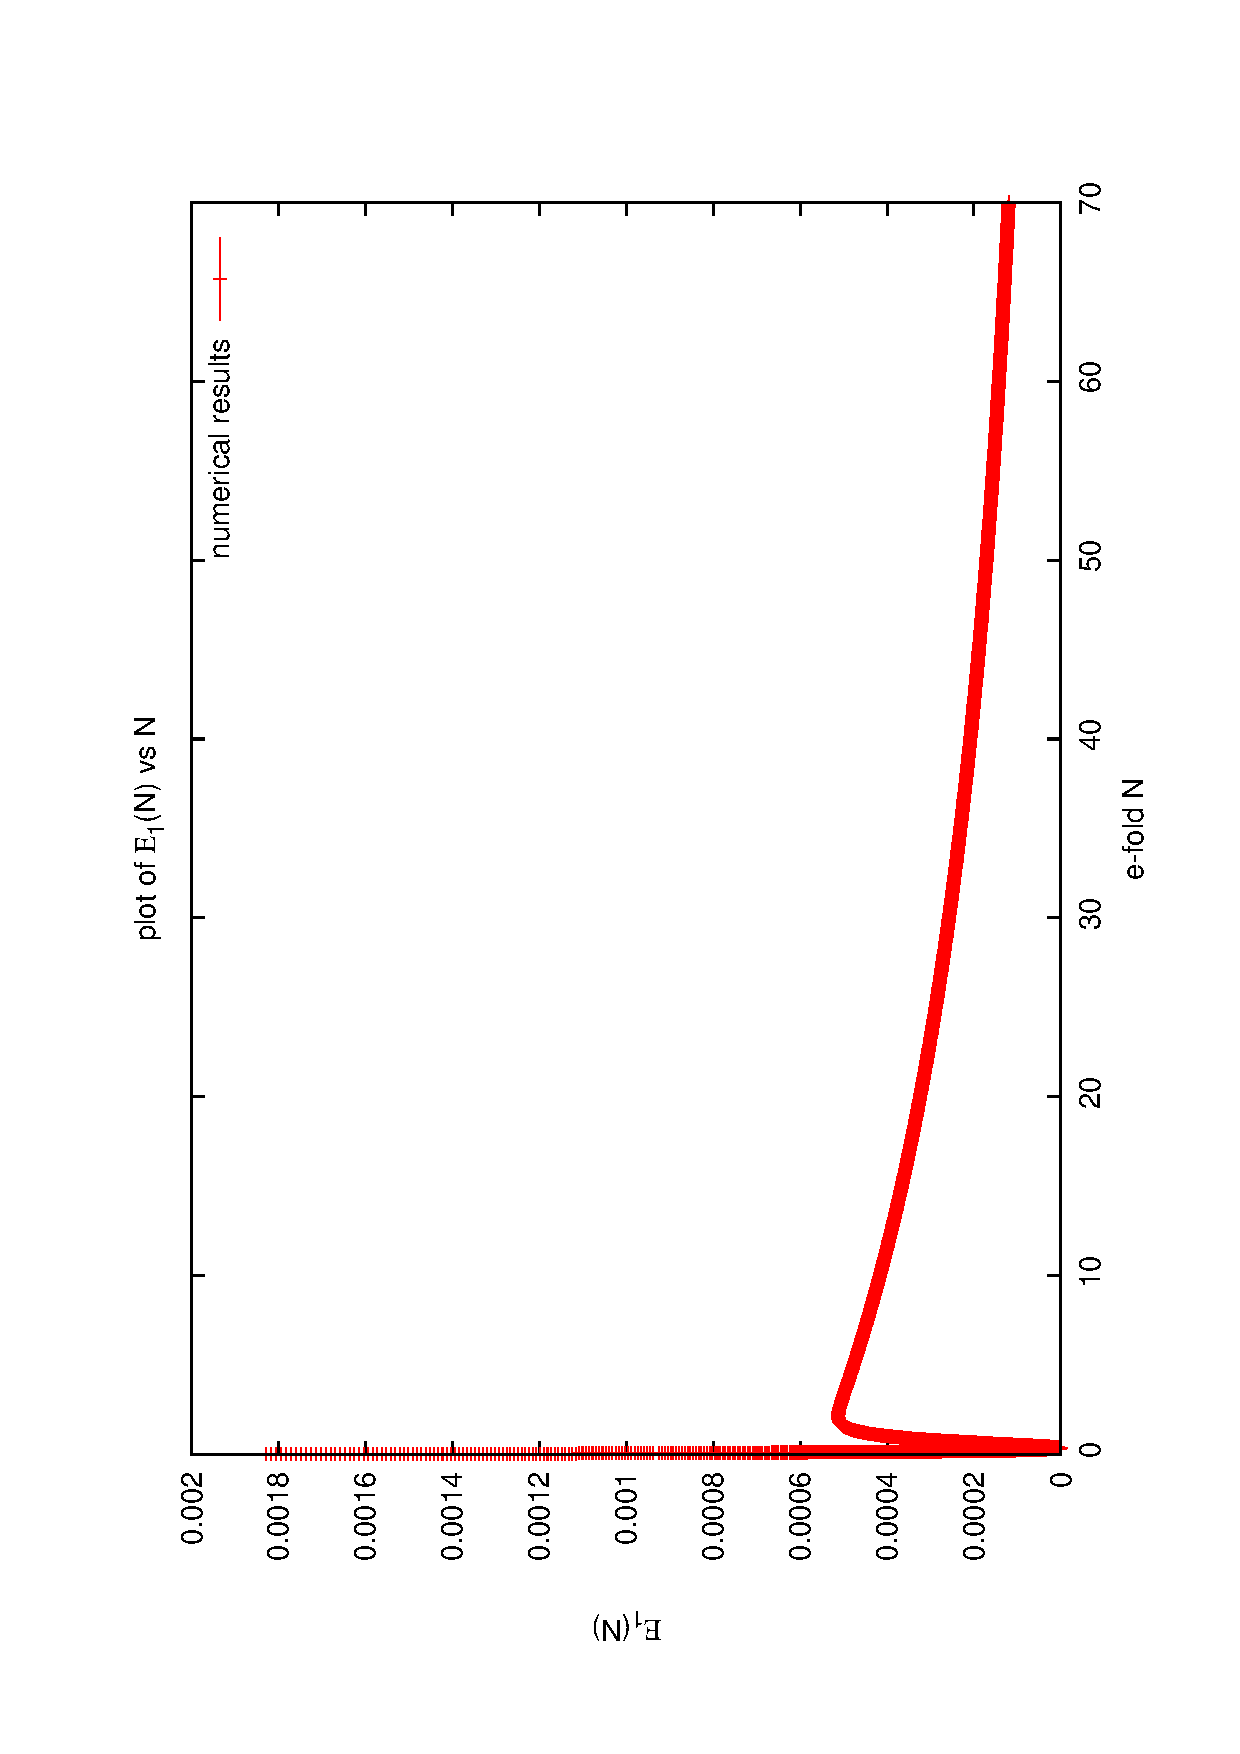
\includegraphics[scale=0.5]{plots/eps1_vs_N_small_field.png}
\end{frame}

\begin{frame}
\includegraphics[scale=0.5]{plots/power_spectrum_small_field.png}
\end{frame}

\begin{frame}{A sample slide}

A displayed formula:

\[
  \int_{-\infty}^\infty e^{-x^2} \, dx = \sqrt{\pi}
\]

\pause
An itemized list:

\begin{itemize}
  \item itemized item 1
  \item itemized item 2
  \item itemized item 3
\end{itemize}

\pause
\begin{theorem}
  In a right triangle, the square of hypotenuse equals
  the sum of squares of two other sides.
\end{theorem}

\end{frame}

\begin{frame}
  \frametitle{Splitting a slide into columns}

The line you are reading goes all the way across the slide.
From the left margin to the right margin.  Now we are going
the split the slide into two columns.
\bigskip

\begin{columns}[t]

\pause
  \begin{column}{0.5\textwidth}
    Here is the first column.  We put an itemized list in it.
    \begin{itemize}
      \item This is an item
      \item This is another item
      \item Yet another item
    \end{itemize}
  \end{column}

\pause
  \begin{column}{0.3\textwidth}
    Here is the second column.  
    \end{column}
\end{columns}
\bigskip

\pause
The line you are reading goes all the way across the slide.
From the left margin to the right margin.

\end{frame}

\begin{frame}{Last Page}
Click \hyperlink{cover}{here} to go to the cover
\end{frame}

\end{document}